\documentclass[fontsize=10pt,paper=b5,open=any,
twoside=no,toc=listof,toc=bibliography,headings=optiontohead,
captions=nooneline,captions=tableabove,english,DIV=15,numbers=noenddot,final,parskip=half-,
headinclude=true,footinclude=false,BCOR=0mm]{scrartcl}
\pdfvariable suppressoptionalinfo 512\relax
\synctex=1

\author{Valentin Boettcher, Bill Coish}
\usepackage{hirostyle}
\usepackage{hiromacros}
\addbibresource{references.bib}

\title{The non-Markovian Quantum Walk for Finite Baths (Summary)}
\date{May 26, 2023}
\graphicspath{{plots}}


\begin{document}
\maketitle
Herein we report how to reproduce the behavior found for non-Markovian
quantum walk in the continuum limit with the Born approximation
presented in \refcite{Ricottone2020} using a finite number of
reservoir states and a finite coupling strength. The final result is
presented in \cref{fig:example_finite_vs_continuum}. We introduce the
details of the model and explain how
\cref{fig:example_finite_vs_continuum} was produced.
\begin{figure}[H]
  \centering
  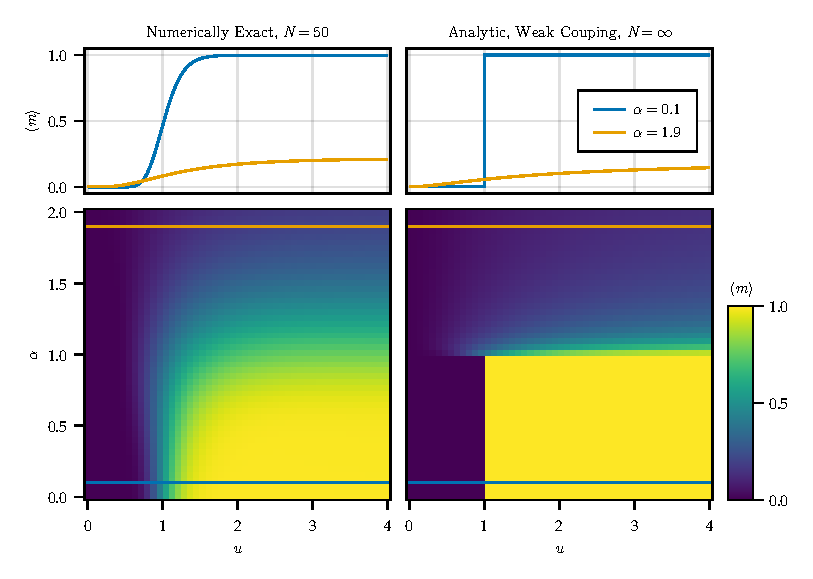
\includegraphics{plots/example_finite_vs_continuum}
  \caption{\label{fig:example_finite_vs_continuum} The full phase
    diagram and constant-\(α\) cuts obtained through numerical
    diagonalization for \(N=50\) reservoir modes and though an
    analytic calculation in the weak coupling limit for \(N\to
    ∞\). All plots shown assume a coupling strength for
    \(g_{0}=0.2 ω_{c}\). Here \(\ev{m}\) is the long-time
    time-averaged walker displacement, \(u=v/v\prime\) is the ratio of
    the inter-cell to intra-cell hopping amplitudes of the underlying
    SSH model, and \(α\) characterizes the bath spectral density
    \(J(ω)\sim ω^{α}\).}
\end{figure}

The basic model is given by~\cite{Ricottone2020}
\begin{align}
  \label{eq:58}
  H &= H_{A} +H_{\bar{A}} + V\\
  H_{A} &= ∑_{m=0}^{L-1}ε_{A} a_{A,m}^{†}a_{A,m} \\
  H_{\bar{A}} &= ∑_{m=0}^{L-1}{(ε_{A} + ω)a_{B,m}^{†}a_{B,m}}+
                   ∑_{j}\bqty{ε_{j} b_{j,m}^{†}b_{j,m} + g_{j}
                   \pqty{a_{B,m}^{†}b_{j,m} + \hc}}\\
  V&=∑_{m=0}^{L-1} v\pqty{a_{A,m}^{†}a_{B,m}+ u a_{A,m}^{†}a_{B,m+1}} + \hc,
\end{align}
which describes an SSH chain with \(L\) sites, periodic boundary
conditions, site energy detuning \(ω\) and extra ``reservoir'' modes
\(b_{j,m}\) in each unit cell that are coupled to the \(B\) sites. We
are using second quantized notation here, where
\(a^{†}_{X,m}\ket{0} = \ket{X,m}\) creates a particle at sublattice
site \(X\) and lattice site \(m\) and
\(b^{†}_{j,m}\ket{0} = \ket{j,m}\) creates a particle in the \(j\)th
reservoir mode at site \(m\). The \(a\) and \(b\) operators obey the
usual bosonic commutation relations. This is equivalent to the single
particle picture in \refcite{Ricottone2020}, as this Hamiltonian
preserves excitations.

We are interested in the evolution of an initial state of a particle,
the ``walker'', \(\ket{\psi(0)}=\ket{A,0}\) with respect to the
parameter \(u\) and the structure of the reservoir, namely the choice
of \(ε_{j}\) and \(g_{j}\). An observable that is sensitive to the
bath structure \emph{and} the topological phase of the SSH bare
model\footnote{This is understood as setting \(g_{j}=0\) and \(ω=0\)
  leaving \(v\) and \(u\) unchanged.} is the mean displacement
\begin{equation}
  \label{eq:59}
  \ev{m(t)} \equiv ∑_{m}m {ρ_{\bar{A},m}(t)}
\end{equation}
where
\(ρ_{\bar{A},m}(t) = {∑_{l\neq A} \abs{\braket{l,m}{ψ(t)}}^{2}}\) is
the probability that the walker does reside in cell \(m\) but not the \(A\) site in
cell \(m\) at time \(t\).

To simplify calculations, we exploit the translational symmetry of the
model to express it in momentum space and remove the \(B\) sites by a
Schrieffer-Wolff transformation for large \(ω\) resulting in
\(H=∑_{k}H(k)\) with
\begin{equation}
  \label{eq:61}
  H(k) = {ω}_{A} a_{A,k}^{†}a_{A,k}+ ∑_{j} \bqty{{ω}_{j} b_{j,k}^{†}b_{j,k}
    + \pqty{\frac{v(k)}{\abs{v(0)}}η_{j} a_{A,k}^{†}b_{j,k}+ \hc}},
\end{equation}
where \(k=\frac{2π n}{L}\) for \(n\in[0, L-1]\), \(L\in\NN\),
\(c_{l,k} = \frac{1}{\sqrt{L}}∑_{m}c_{l,m}\eu^{-\iu k m}\) and
\begin{equation}
  \label{eq:72}
  v(k)=v+v\prime\eu^{\iu k}=v(1+u)\eu^{\iu k} = \abs{v(k)}\eu^{\iu ϕ(k)}.
\end{equation}


The mean displacement can be re-expressed in terms of momentum space quantities
\begin{equation}
  \label{eq:62}
  \begin{aligned}[t]
  \ev{m(t)} &= ∑_{k} \pqty{\frac{1}{L}-ρ_{A}\pqty{k,
              t}}\dv{ϕ({k})}{k}
  \end{aligned}
\end{equation}
where \(ρ_{A}(k,t)=\abs{\braket{A,k}{ψ(t)}}^{2}\) with
\(\ket{ψ(0)}=\ket{A,k=0}=a^{†}_{A,k=0}\ket{0}\).

The structure of the reservoir is described by the
spectral density which we choose to take the form of a power law
\begin{equation}
  \label{eq:64}
  J(ω)
  =
  \begin{cases}
    \pqty{g_{0}^{2}\frac{(α+1)}{ω_{c}^{α+1}}} ω^{α} & \mathrm{for}\; 0\leq
                                               ω\leq ω_{c}\\
    0 & \mathrm{otherwise},
  \end{cases}
\end{equation}
where \(ω_{c}\) is called the cutoff frequency and \(α\) controls how
fast \(J(ω)\) approaches zero for \(ω\to 0\). The coupling strength
\(g_{0}\) can be expressed by the couplings through
\begin{equation}
  \label{eq:70}
  g_{0} = \sqrt{∑_{j}\abs{η_{j}}^{2}}.
\end{equation}
For finite-size reservoirs, a simple choice for the \(ω_{j}\) and
\(η_{j}\) is
\begin{equation}
  \label{eq:65}
  \begin{aligned}
    Δω &= \frac{ω_{c}}{N} & ω_{j} &= Δω \pqty{j + \frac{1}{2}} & η_{j}^{2}
    &= J(ω_{j}) Δω,
  \end{aligned}
\end{equation}
which recovers \cref{eq:64} in the limit \(N\to ∞\).

The finite size of the reservoir will in general wash out the sharp
phase transitions observed in \refcite{Ricottone2020}. Additionally it
will lead to recurrences in the dynamics around the time
\begin{equation}
  \label{eq:71}
  τ_{R}=\frac{2π}{Δω},
\end{equation}
where \(N\) is the number of reservoir modes. This means, that around
\(τ_{R}\), the state of the system will approach initial state. As we
are interested in reproducing the behavior of the infinite system, we
have to work on time-scales where this effect doesn't come to play.

On the other hand
\(ρ_{A}(k,t)\) decays with a rate
\begin{equation}
  \label{eq:1}
  Γ \sim \frac{π g_{0}^{2}}{ω_{c}}.
\end{equation}
It is therefore necessary to have \(1/Γ \ll τ_{R}\), which gives a
lower bound for the number of reservoir states required at a certain
coupling strength
\begin{equation}
  \label{eq:73}
  N \gg \frac{ω_{c}^{2}}{2π^{2}g_{0}^{2}} .
\end{equation}

Further, the strong coupling limit where
\(\ev{m(t)}\sim \cos[2](Ω t)\) with \(Ω=\sqrt{∑_{j}\abs{η_{j}}^{2}}\)
should be avoided, which adds the constraint
\begin{equation}
  \label{eq:2}
  g_{0}^{2} \ll ω_{c}^{2}.
\end{equation}

To define the time averaged displacement for a finite reservoir, we
have to avoid transients and revivals, yielding
\begin{equation}
  \label{eq:69}
  \ev{m} \equiv \frac{1}{τ_{h} - τ_{l}} ∫_{τ_{l}}^{τ_{h}}\ev{m(t)} \dd{t},
\end{equation}
with \(τ_{l}\) and \(τ_{h}\) chosen appropriately to avoid transient
and recurrences, but far enough apart to provide a satisfactory
average. A reasonable choice would be
\(τ_{l}=0.5 τ_{R},\, τ_{h} = 0.95 τ_{R}\).

In the continuum limit we can ignore transient effects and choose
\(τ_{l}=0\) and take the limit of \(τ_{h}\to ∞\) obtaining
\begin{equation}
  \label{eq:60}
  \ev{m} =  \lim_{T\to ∞} \frac{1}{T} ∫_{0}^{T}\ev{m(t)}\dd{t}.
\end{equation}

If \(ρ_{A}(k,t)\xrightarrow{t\to ∞}0\) for all \(k\), the long-time
averaged mean displacement \(\ev{m}\) exhibits a universal behavior
corresponding to the topological phase of the original SSH chain
\begin{equation}
  \label{eq:63}
  \ev{m} = θ(u-1).
\end{equation}
It was shown in \refcite{Ricottone2020} using the Born approximation
and taking the continuum limit for the reservoir and an infinite SSH
chain \(L=∞\), that \(\ev{m}\) matches \cref{eq:63} precisely for
\(α<1\) whereas it takes on non-universal values for \(α>1\). This
behavior can also be obtained without employing the Born approximation
and is presented in the right column of
\cref{fig:example_finite_vs_continuum}.

If we choose \(g_{0}=0.2\implies g_{0}^{2}=0.04\), we are just about
fulfilling \cref{eq:2}, while \cref{eq:73} evaluates to
\(N\gtrsim 1\). The resulting \(\ev{m(t)}\) for \(N=50\) and \(α=0.1\)
and \(u=4\) is shown in \cref{fig:mean_displacement_example}, where we
see that the time scales are indeed well separated and \(\ev{m}\)
approaches the value one as we would expect from the weak coupling and
continuum limit.
\begin{figure}[H]
  \centering
  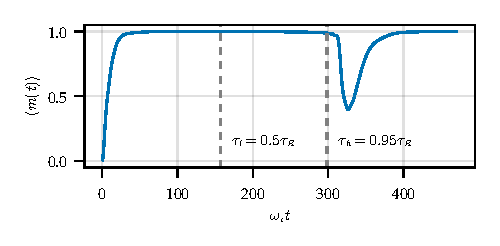
\includegraphics[width=.8\linewidth]{plots/mean_displacement_example_simple}
  \caption{\label{fig:mean_displacement_example} The mean \(\ev{m}\)
    displacement over time for two values of \(α\), \(u=4\), \(N=50\)
    in relation to the recurrence time \(τ_{R}\).}
\end{figure}

In choosing a non-vanishing \(g_{0}>0\) we have to compensate for
level repulsion which shifts the effective energy of the \(A\) site.
This Lamb shift can be countered by choosing a specific value of the
\(A\) site energy
\begin{equation}
  \label{eq:66}
  ω_{A} = ∑_{j}\frac{\abs{η_{j}}^{2}}{ω_{j}} = \frac{1}{N} ∑_{j}
  J(ω_{j}) \frac{ω_{c}}{ω_{j}},
\end{equation}
where \(ω_{A}\) is independent of \(u\) but still depends on
\(α\). This was done to produce
\cref{fig:mean_displacement_example,}.


The full phase diagram for the finite reservoir is presented on the
left side of \cref{fig:example_finite_vs_continuum}. While finite size
effects wash out the sharp borders of the phase diagram in the
continuum limit, its signature is relatively clear, especially in the
constant \(α\) cuts above the phase diagram.


\printbibliography{}
\end{document}


%%% Local Variables:
%%% mode: latex
%%% TeX-master: t
%%% TeX-output-dir: "output"
%%% TeX-engine: luatex
%%% End:
